\documentclass{article}
\usepackage{graphicx}
\usepackage{amsmath}
\usepackage{float}
\usepackage{qcircuit}
\usepackage{hyperref}
\usepackage{graphicx}
\usepackage{rotating}
\usepackage{pdflscape}
\usepackage{multirow,tabularx}
\usepackage{authblk}
\usepackage{amsthm}
\usepackage{caption}
\usepackage{subcaption}
\usepackage{tabularx}
\usepackage{cite}
\usepackage{color}

\begin{document}

\section{IBM Q2 and the Hard Mapping Problem}
IBM recently has provided the world with one of the first quantum computers. Even though it is not one of the powerful quantum computers available in the market, but it has proven the world it is possible to construct such devices. Unfortunately, this quantum computer comes with very restrictive interactions. Take for example the \textit{IBM Q2} illustrated in Figure \ref{fig:ibmq2}, it has restrictions on the interactions between qubits. For example, $Q0$ can be the control qubit for $Q1$ and $Q2$; $Q2$ can be the target qubit for both $Q0$ and $Q1$. $Q1$ can be both a target qubit and a control qubit; i.e. the arrows depicted in Figure \ref{fig:ibmq2} illustrate the restrictions of interactions between qubits.


Given the circuit in Figure \ref{fig:exercise1}, map it on IBM Q2 using as minimum quantum gates as possible.You may use the variations of SWAP gates as a workaround Figure \ref{fig:swap-gates}.

\begin{figure}[H]
    \centering
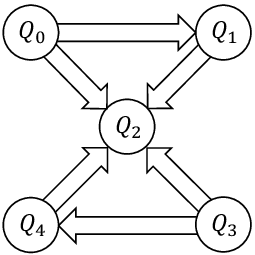
\includegraphics[width=2.5cm, height=2.5cm]{assets/images/The-architecture-of-IBM-Q-Experiences-5-qubit-quantum-computer-IBMQX2-cited-from-20.png}

    \caption{IBM Q2 quantum computer. \label{fig:ibmq2}}
\end{figure}



\begin{figure}[H]
        \begin{align*}
            \Qcircuit @C=1.0em @R=1em @!R{
               \lstick{x_0} &\qw&\qw&\targ&\qw&\qw&\qw\\ 
               \lstick{x_1}  &\qw&\qw&\ctrl{ -1 }&\ctrl{ 3 }&\qw&\qw\\ 
               \lstick{x_2}  &\qw&\ctrl{ 1 }&\qw&\qw&\ctrl{ 1 }&\qw\\ 
               \lstick{x_3}  &\qw&\targ&\qw&\qw&\targ&\qw\\ 
               \lstick{x_4}  &\qw&\qw&\qw&\targ&\qw&\qw\\ 
            }
        \end{align*}
        \caption{Map this circuit on \textit{IBM Q2}. \label{fig:exercise1}}
\end{figure}


\begin{figure}[H]
\centering

% \hfill
\begin{subfigure}[b]{0.4\textwidth}
        \begin{align*}
        \Qcircuit @C=1.0em @R=1em @!R{
        &\qw&\gate{H}&\ctrl{ 1 }&\gate{H}&\qw\\ 
        &\qw&\gate{H}&\targ&\gate{H}&\qw\\ 
        }
    \end{align*}

\end{subfigure}
\hfill
\begin{subfigure}[b]{0.4\textwidth}
        \begin{align*}
        \Qcircuit @C=1.0em @R=1em @!R{
            &\qw&\ctrl{ 1 }&\targ&\ctrl{ 1 }&\qw\\ 
            &\qw&\targ&\ctrl{ -1 }&\targ&\qw\\ 
        }
        \end{align*}
\end{subfigure}
\caption{Variations of SWAP gate. \label{fig:swap-gates}}
\end{figure}

    

\section{The John Doe Circuit}
While searching online, to satisfy your sense of curiosity about quantum, you stumped upon the circuit in Figure \ref{}. You're interested to know what computations it perform on the input. Trace this circuit to find the output.

% \begin{figure}[H]
%     \begin{align*}
%         \Qcircuit @C=1.0em @R=1em @!R{


%         }
% \end{figure}


\section{The Jane Doe Black-Box Circuit}
A black-box circuit is a circuit hidden in an unbreakable box which means you cannot open the black-box and see how qubits interact with each other and which gates are used as well,\textit{ i.e.}, everything is hidden from sight. This black-box promises to output certain Boolean functions on every output qubit, given an input. Given the black-box in Figure \ref{fig:jane-doe}, try to reverse-engineer the output to get the circuit that performs this Boolean operations. You may use the gates provided in Figure \ref{}


\begin{figure}[H]
    \begin{align*}
        \Qcircuit @C=1.0em @R=1em @!R{
            \lstick{A}&\qw&\multigate{3}{Jane Doe}&\qw &  \rstick{A}\\ 
            \lstick{B} &\qw&\ghost{Jane Doe}&\qw & \rstick{A\oplus B}\\ 
            \lstick{0} &\qw&\ghost{Jane Doe}&\qw & \rstick{A\oplus B \oplus C}\\ 
            \lstick{C} &\qw&\ghost{Jane Doe}&\qw & \rstick{AB\oplus BC\oplus AB }\\ 
        }
        \end{align*}
        \caption{The Jane Doe Black-box. \label{fig:jane-doe}}
\end{figure}

\begin{figure}[H]
    \begin{subfigure}[b]{0.4\textwidth}
        
        \begin{align*}
            \Qcircuit @C=1.0em @R=1em @!R{
           \lstick{A} &\qw&\ctrl{ 2 }&\qw & \rstick{A}\\ 
           \lstick{B} &\qw&\ctrl{ 1 }&\qw & \rstick{B}\\ 
           \lstick{C} &\qw&\targ&\qw & \rstick{AB\oplus C}\\ 
        }
        \end{align*}
    \end{subfigure}

\hfill
    \begin{subfigure}[b]{0.4\textwidth}
        
        \begin{align*}
            \Qcircuit @C=1.0em @R=1em @!R{
                \lstick{A} &\qw&\ctrl{ 1 }&\qw &  \rstick{A}\\ 
                \lstick{B} &\qw&\targ&\qw & \rstick{A\oplus B}\\ 
            }
            \end{align*}
\end{subfigure}


\end{figure}

\end{document}